\section{ Wirtschaftswachstum}

\subsection{Problemstellung: Warum Wachstum?}

Wenn Wohlstand positiv mit Lebensqualität korreliert, stellt sich die strategische Frage:

\begin{itemize}
    \item Wie kann langfristiger Wohlstand gesteigert werden?
    \item Welche Wachstumsquellen sind politisch beeinflussbar?
    \item Wie entwickelte sich das BIP pro Kopf der Schweiz?
    \item Warum wurde 2004 eine offizielle Wachstumspolitik eingeführt?
\end{itemize}

Wachstum ist im Zielpolygon der Wirtschaftspolitik zentral verankert.

\subsection{Bedeutung des langfristigen Wachstums}

\begin{center}
    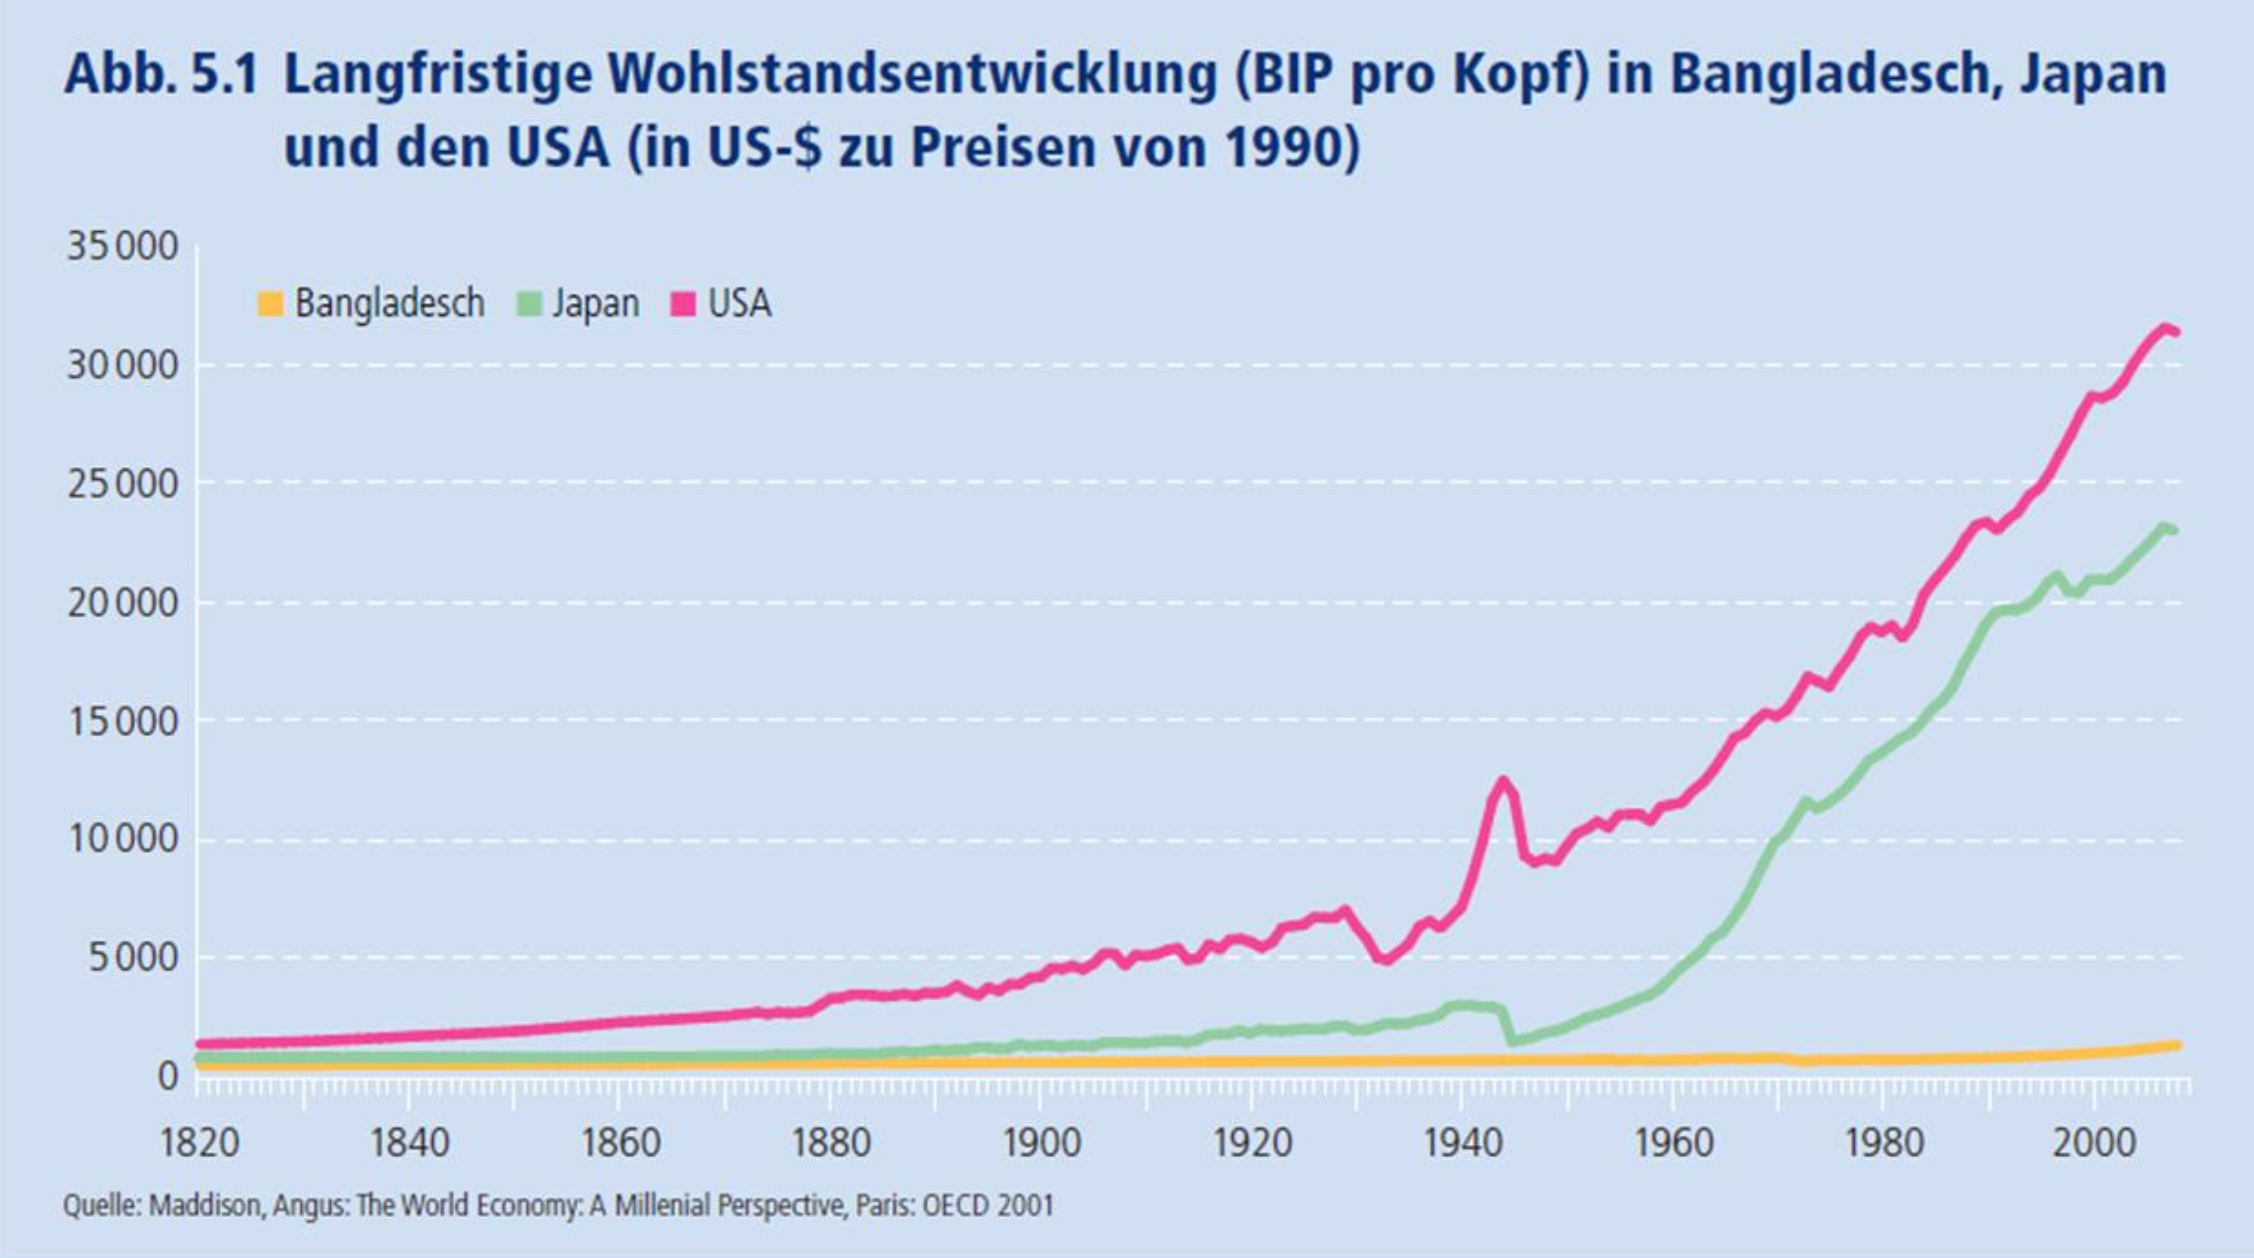
\includegraphics[width=0.8\linewidth]{images/bip_pro_Kopf.png}
\end{center}

Langfristige Unterschiede im Wachstum führen zu massiven Wohlstandsdifferenzen.

Empirischer Vergleich (Bangladesch, Japan, USA):
Kleine Wachstumsunterschiede kumulieren sich exponentiell.

Wachstum erleichtert Verteilung:
Neu geschaffener Wohlstand lässt sich politisch einfacher verteilen als bestehender umzuverteilen.

\subsection{Wachstum vs. Konjunktur}

Unterscheidung:

\begin{itemize}
    \item \textbf{Wachstumstrend:} langfristige Entwicklung des Produktionspotenzials
    \item \textbf{Konjunktur:} kurzfristige Schwankungen um den Trend
\end{itemize}

Konjunktur führt zu Unter- oder Überauslastung.
Langfristiger Wohlstand hängt vom Trend ab, nicht von kurzfristigen Zyklen.

\subsection{Quellen des Wachstums}

\begin{center}
    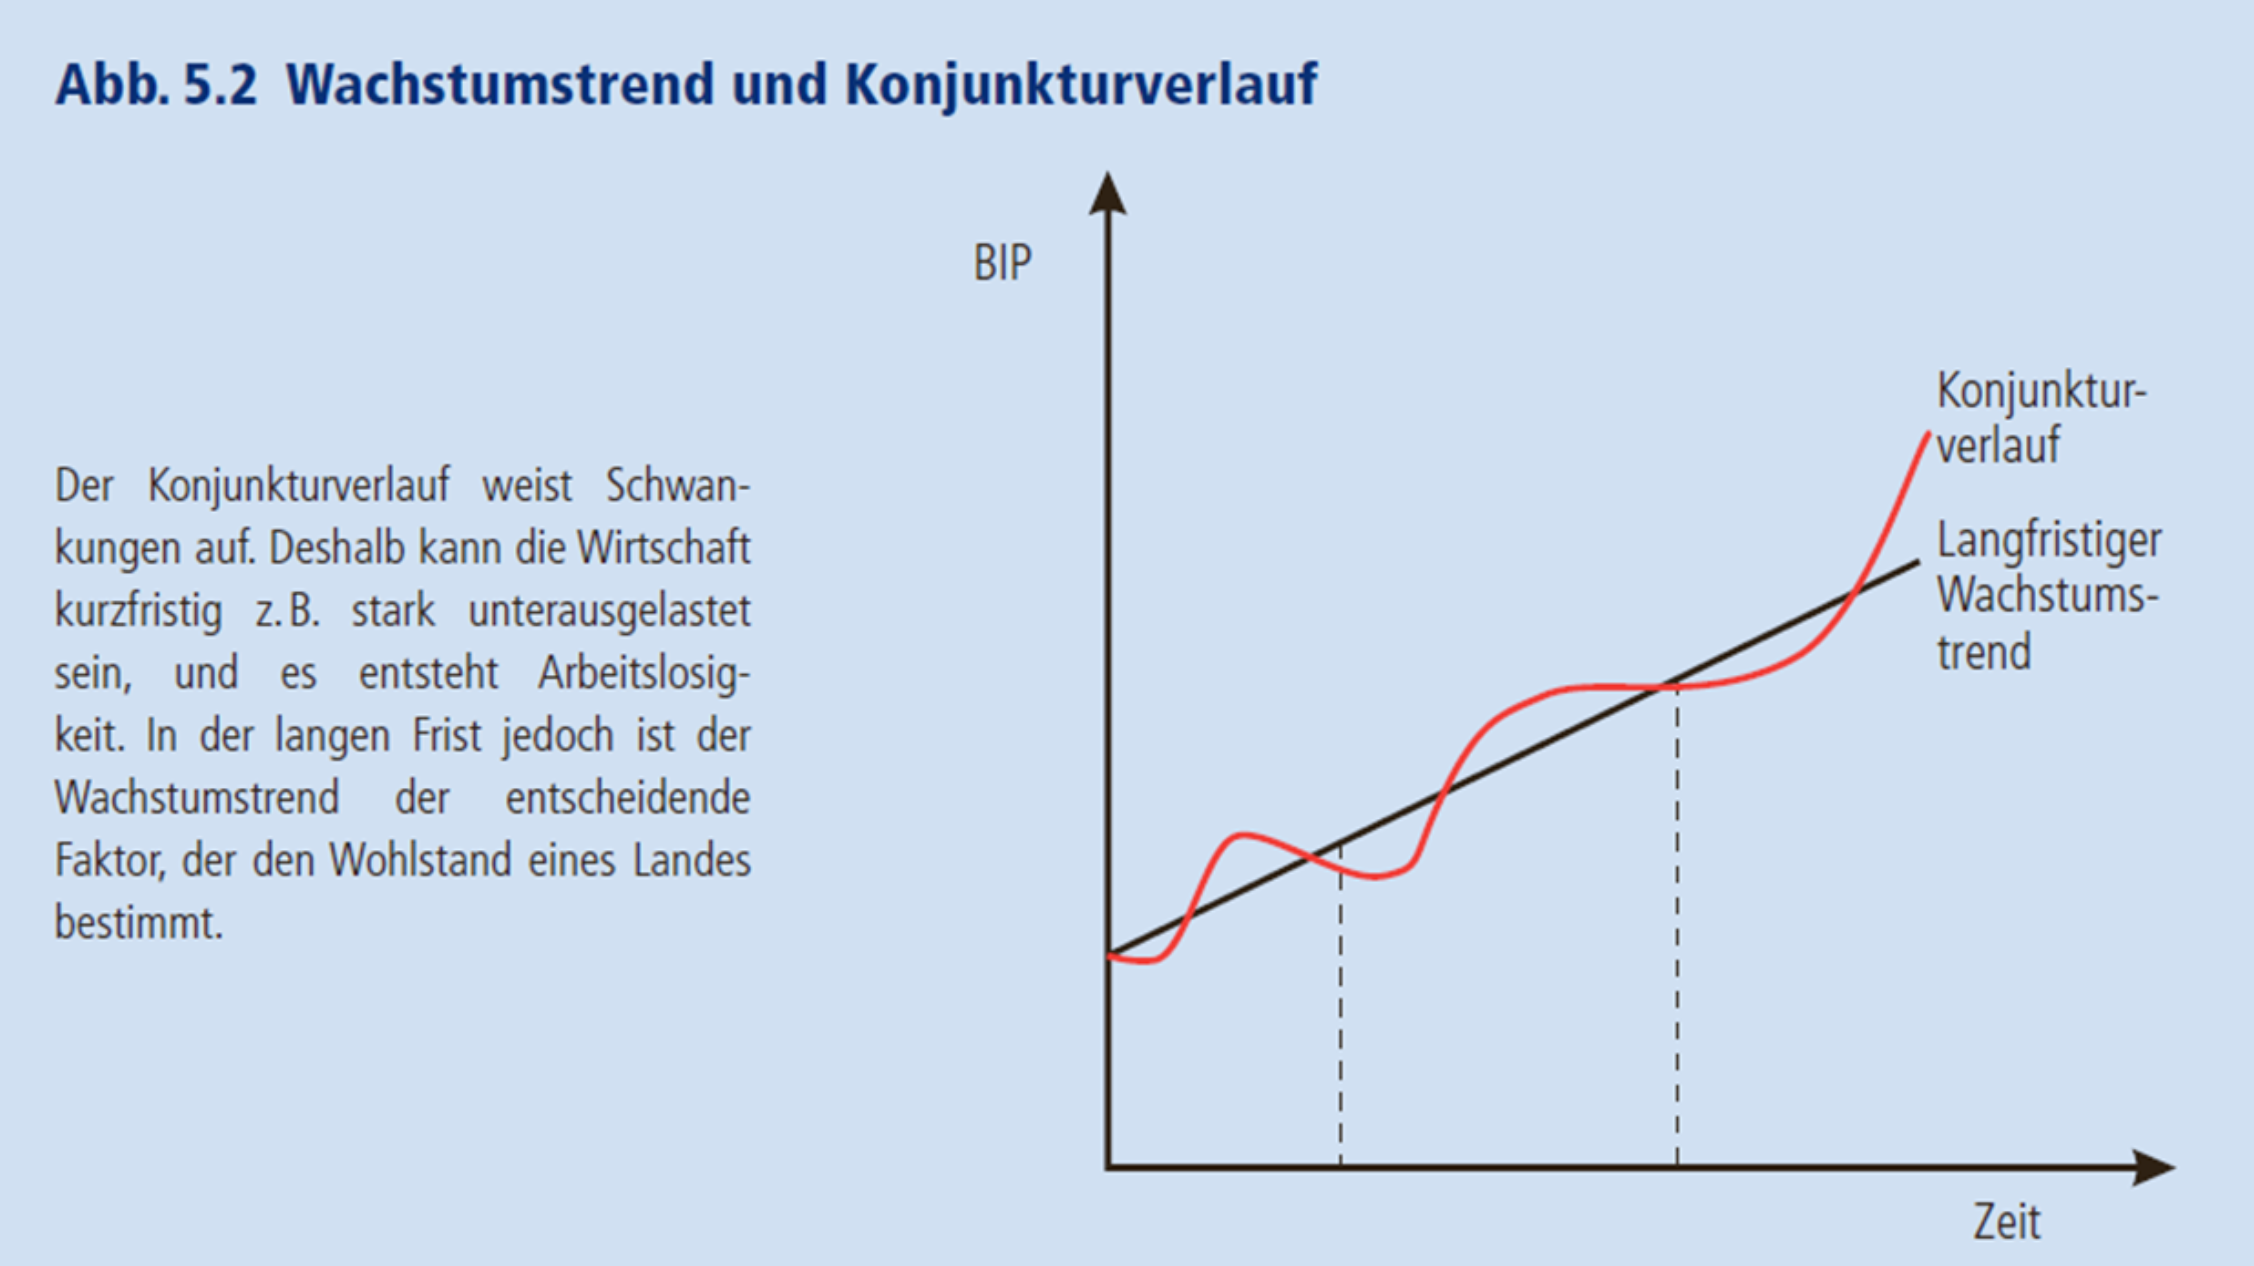
\includegraphics[width=0.8\linewidth]{images/wachstumstrend_konjunkturverlauf.png}
\end{center}

Wachstum des BIP pro Kopf entsteht durch:

\begin{enumerate}
    \item Mehr Arbeitsstunden
    \item Höhere Produktion pro Arbeitsstunde (Arbeitsproduktivität)
\end{enumerate}

\begin{center}
    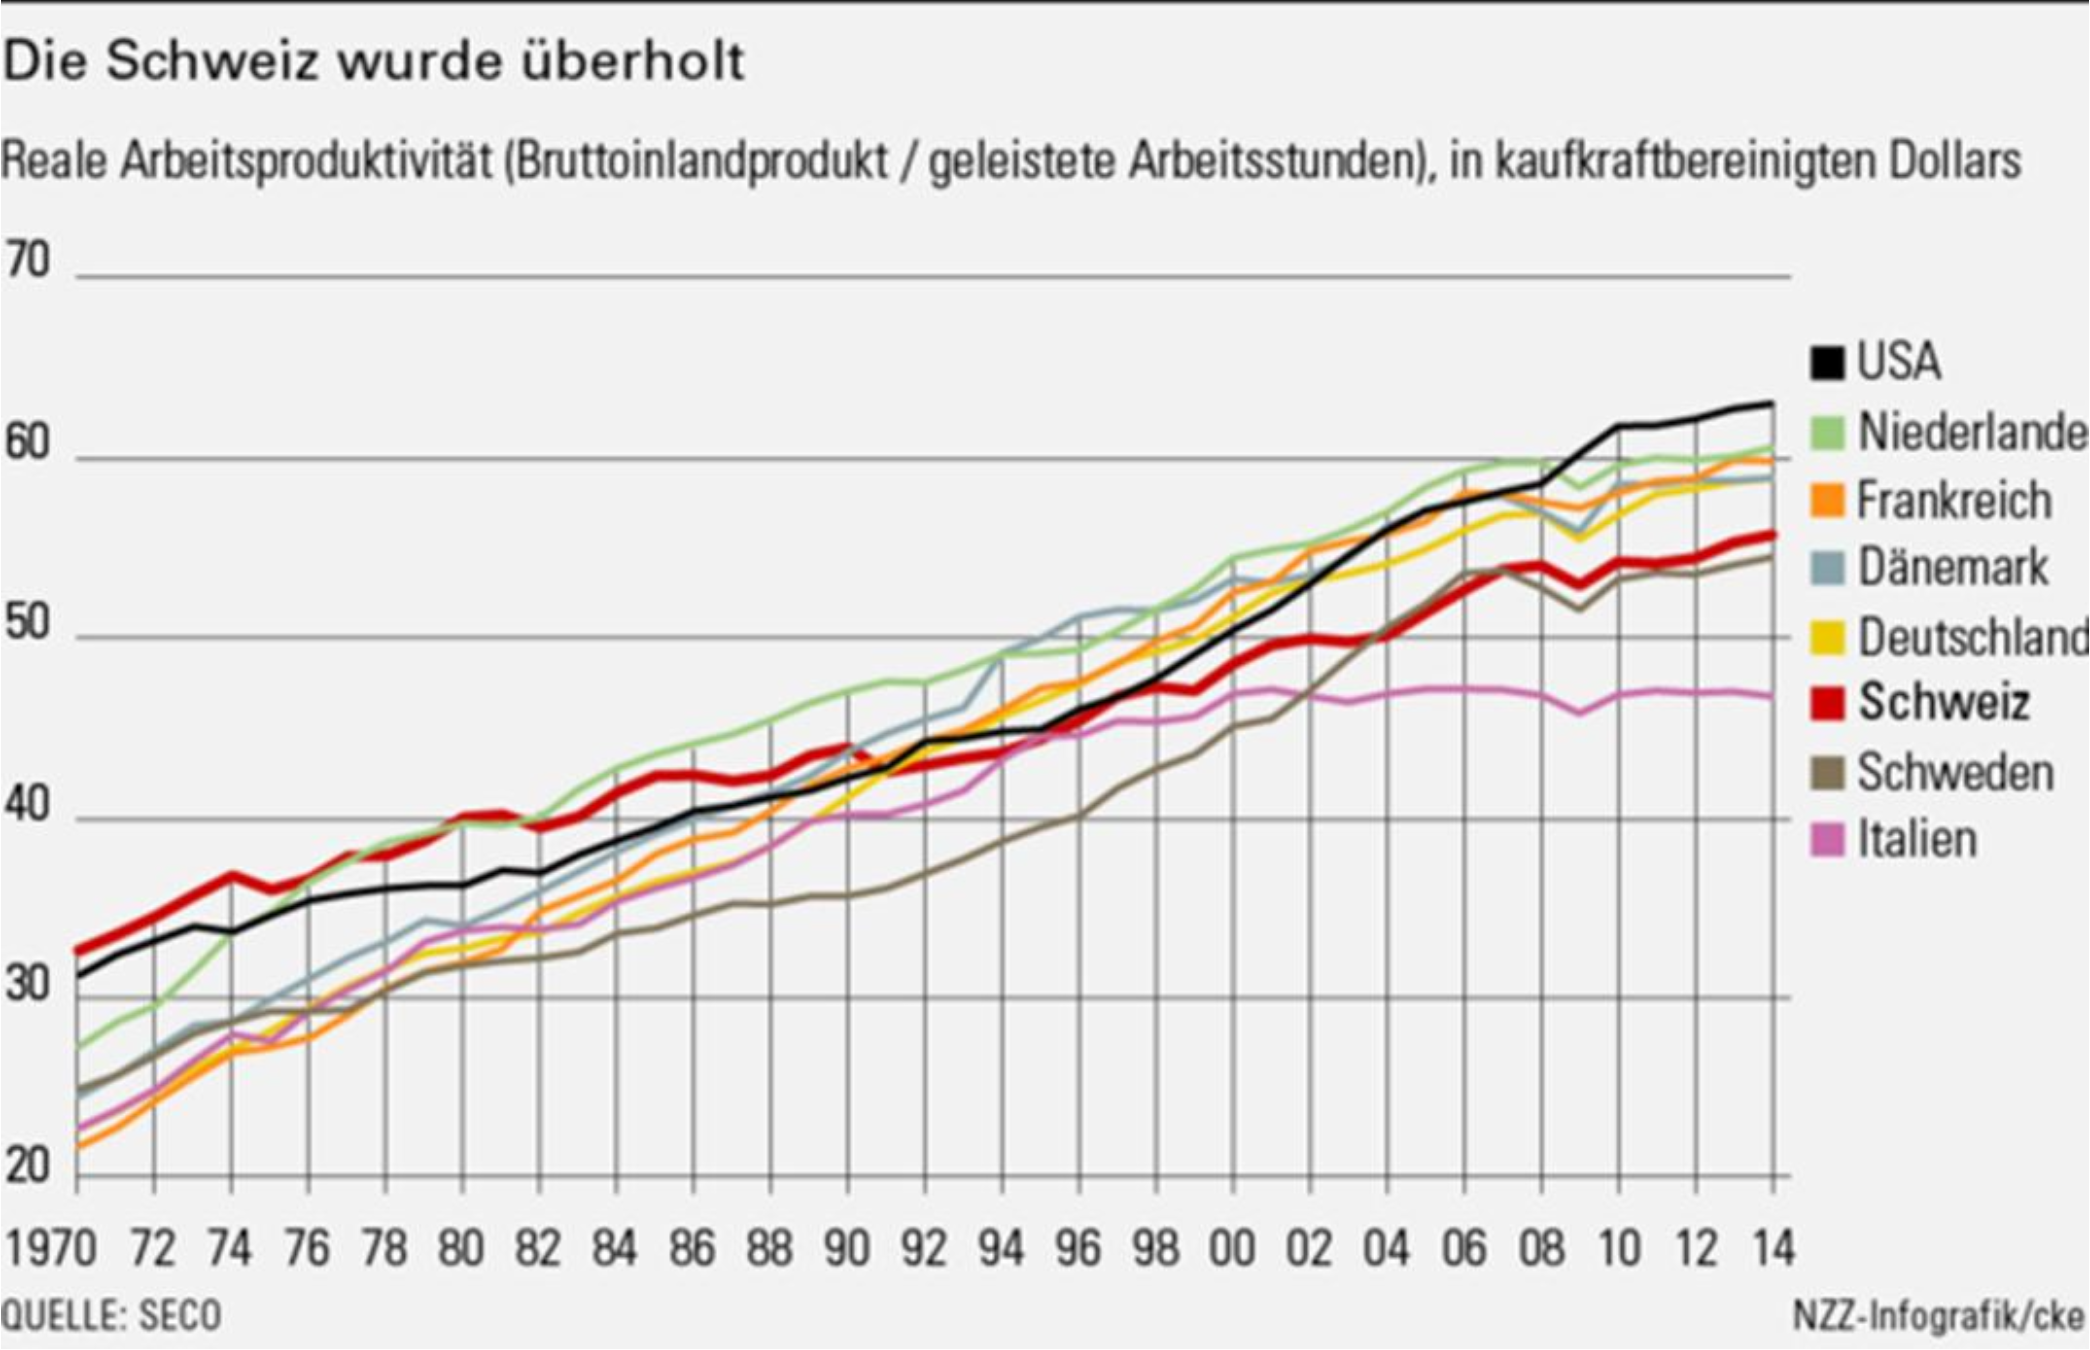
\includegraphics[width=0.8\linewidth]{images/arbeitsproduktivitaet.png}
\end{center}
Produktionsfunktion:
\[
Y = F(K, L, A)
\]

Determinanten:

\begin{itemize}
    \item Mehr Erwerbstätige
    \item Mehr Arbeitsstunden pro Erwerbstätigen
    \item Mehr Realkapital (Investitionen)
    \item Mehr Humankapital (Bildung)
    \item Mehr Know-how (technischer Fortschritt)
\end{itemize}

Langfristig dominiert Produktivitätswachstum.

\begin{center}
    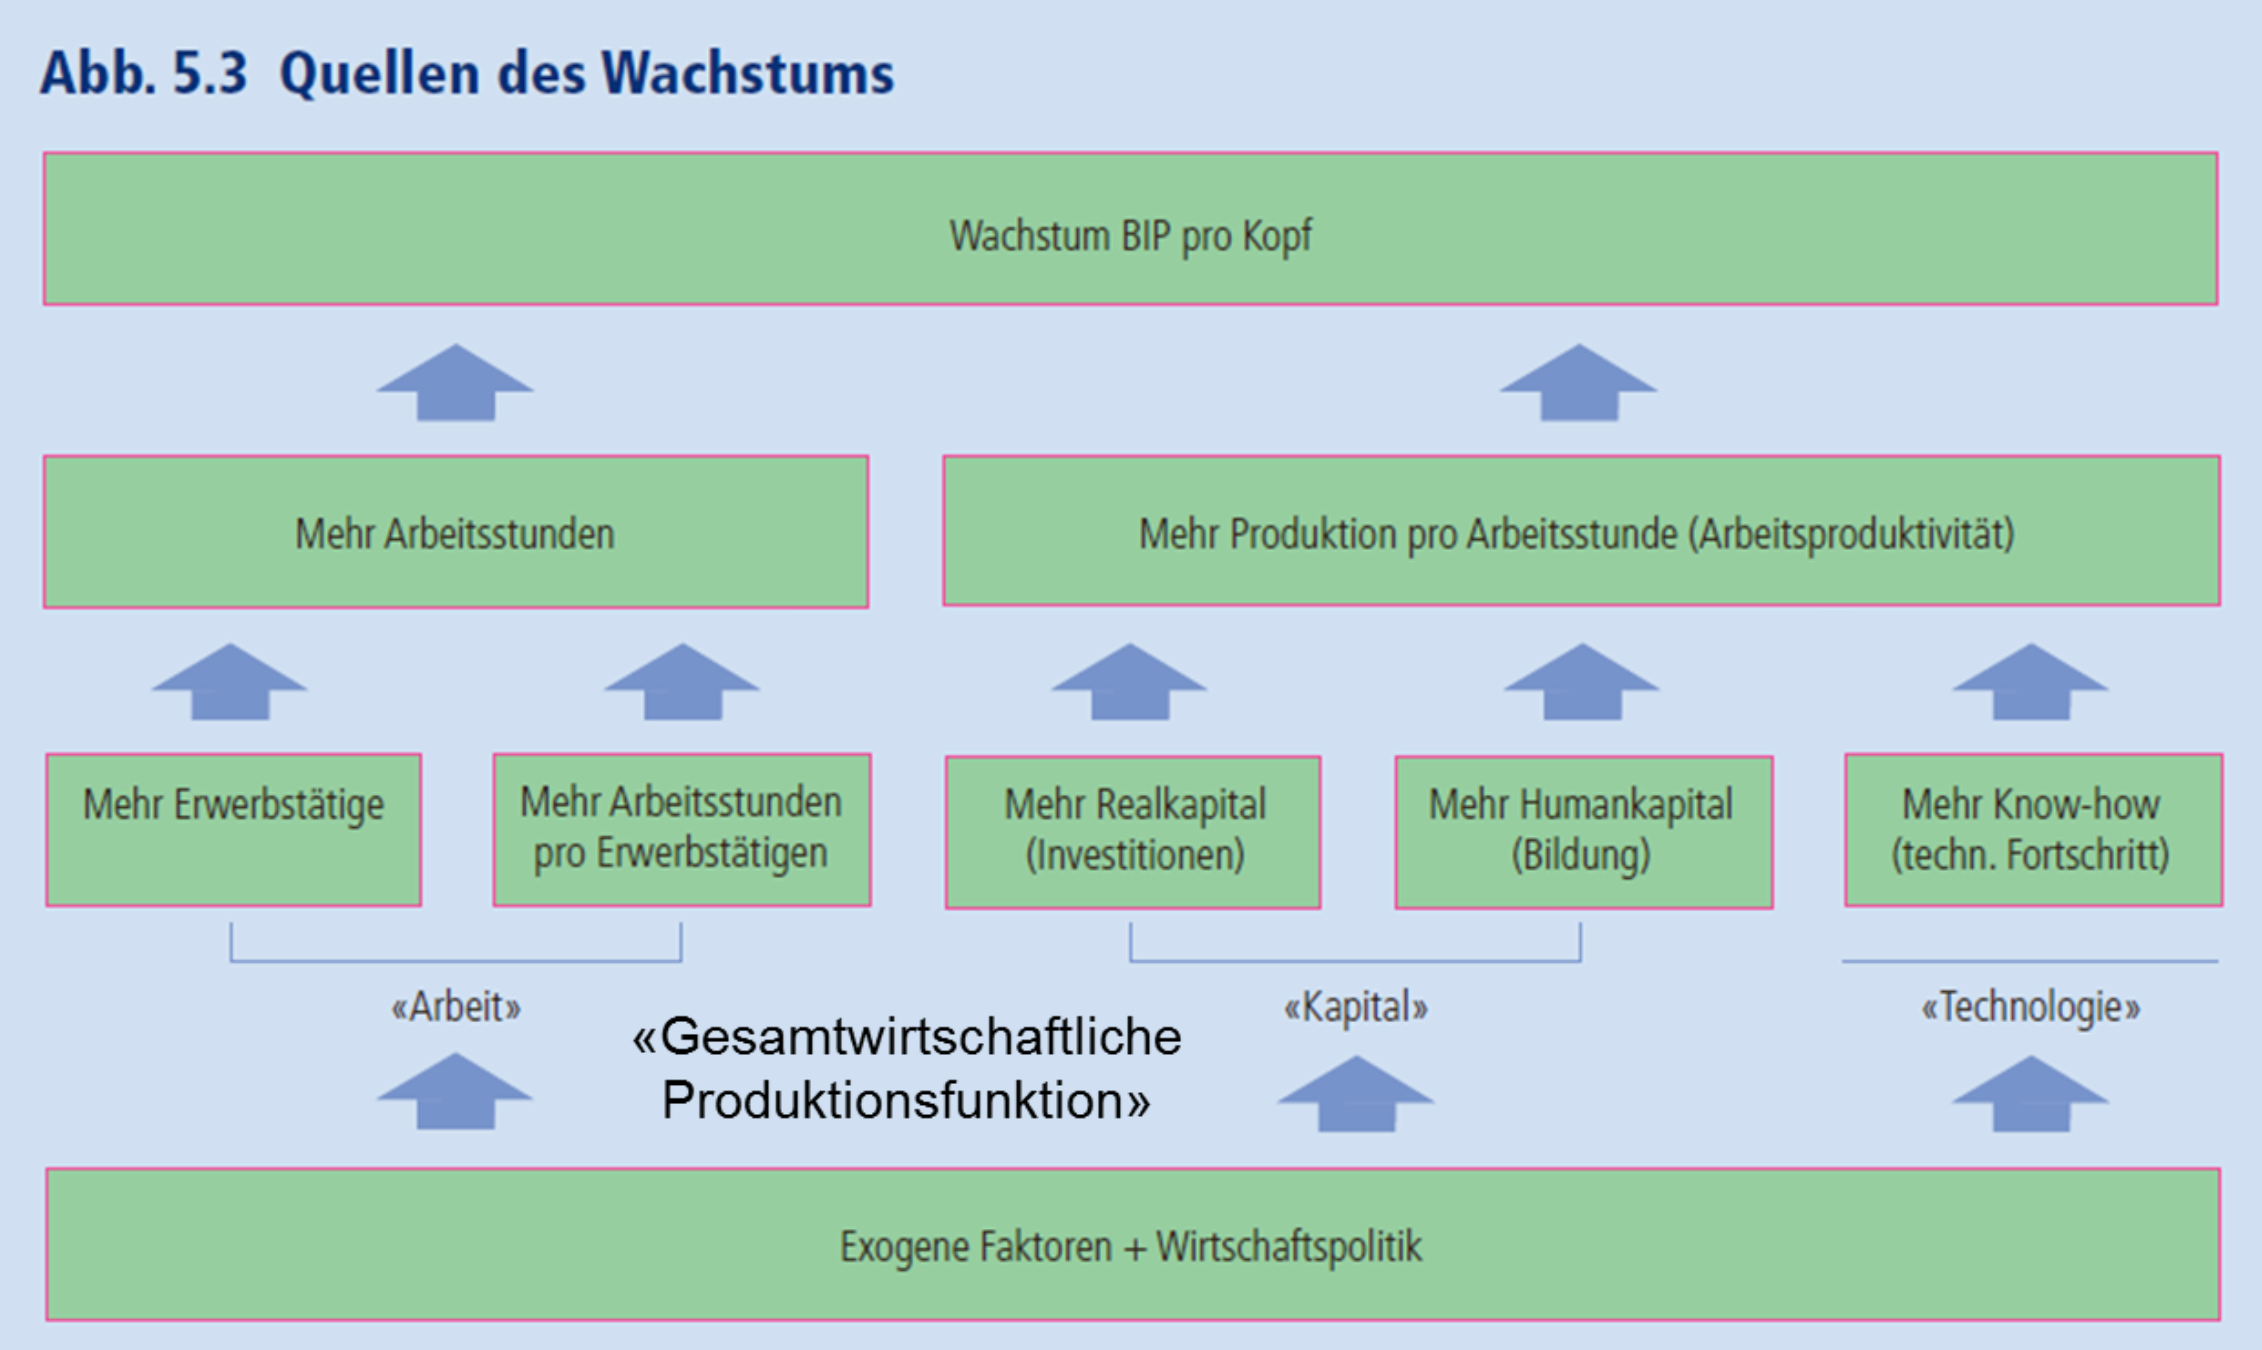
\includegraphics[width=0.8\linewidth]{images/quelle_wachstum.png}
\end{center}

\subsection{Wachstumsentwicklung Schweiz}

Drei historische Phasen:

\begin{itemize}
    \item Phase 1: Moderates Wachstum bis ca. 1950
    \item Phase 2: Starkes Wachstum (Nachkriegsboom)
    \item Phase 3: Deutliche Verlangsamung ab 1970er
\end{itemize}

\begin{center}
    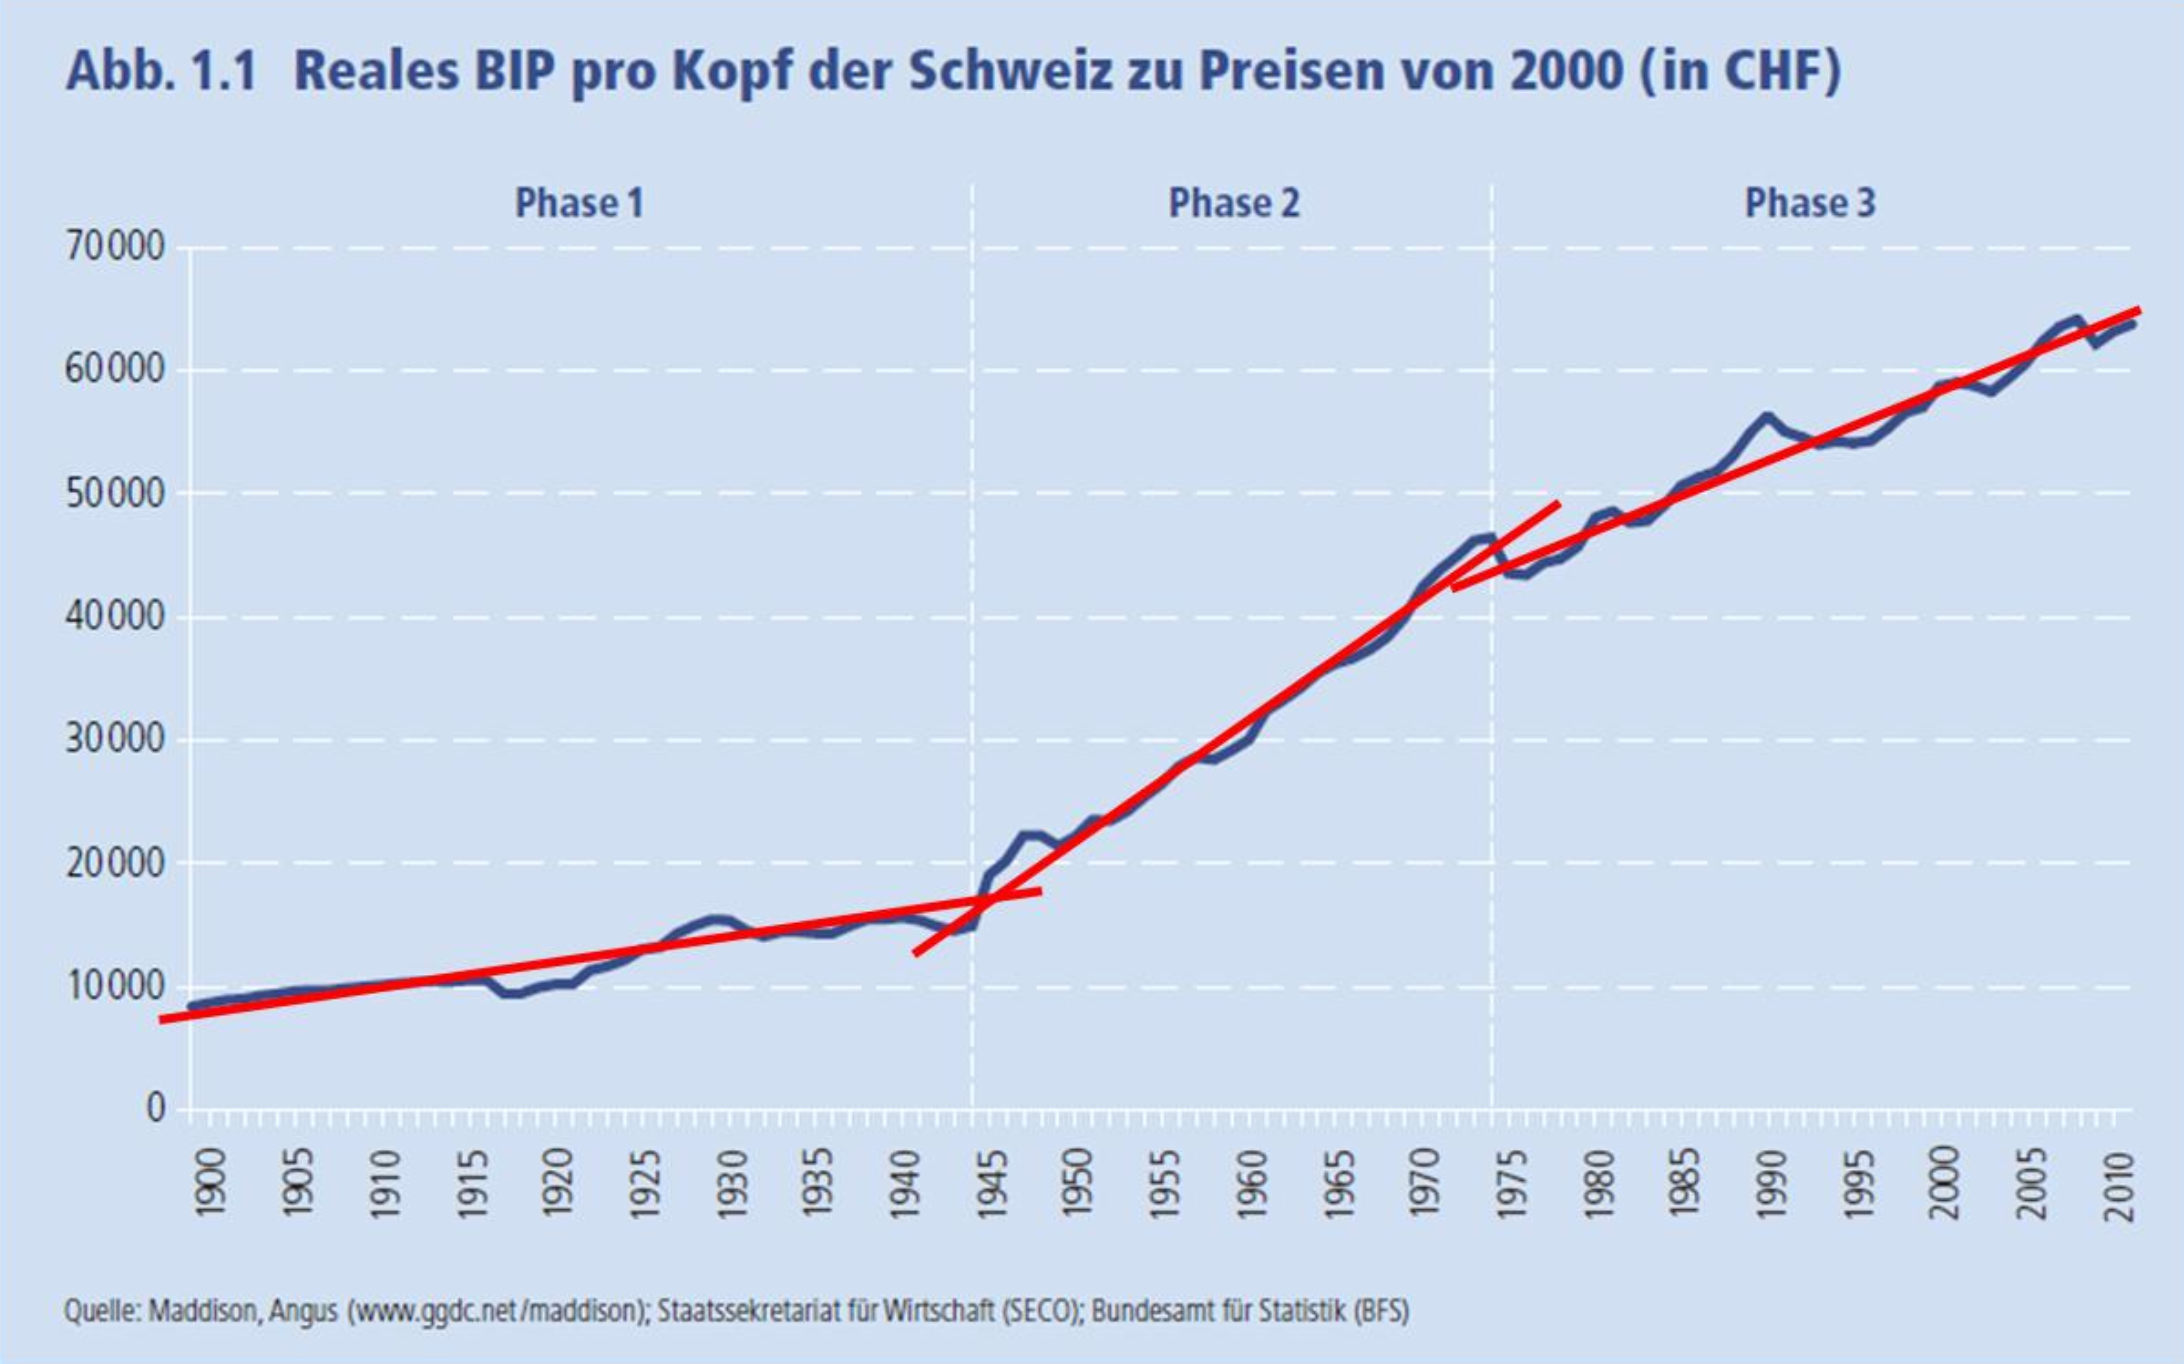
\includegraphics[width=0.8\linewidth]{images/realesbip.png}
\end{center}

Seit den 1990er-Jahren: strukturelle Wachstumsflaute.

\subsection{Diagnose Wachstumsflaute}

Fragestellung:
Liegt die Ursache bei den Arbeitsstunden oder bei der Produktivität?

Analyse zeigt:
Hauptproblem = stagnierendes Produktivitätswachstum.

\subsection{Internationale Produktivitätsvergleiche}

Die Schweiz wurde in Rankings überholt.
Produktivitätswachstum 1995–2014:

\begin{itemize}
    \item Schweiz: ca. 1.2\% pro Jahr
    \item Vergleichsländer teilweise deutlich höher
\end{itemize}

Kleine jährliche Differenzen führen langfristig zu erheblichen Abständen.

\subsection{Mögliche Ursachen der Produktivitätsschwäche}

Die Ursache ist das Wachstum der Staatsquote, insbesondere auch die abschottung des Binnenmarkts( vor allem Landwirtschaft, Energie , Telekommunikation).


\subsection{Rolle der Staatsquote}

These: Expansion staatsnaher Sektoren belastet Produktivitätswachstum.

Beobachtungen:

\begin{itemize}
    \item Starkes Beschäftigungswachstum im öffentlichen Sektor
    \item Geringere Produktivitätsdynamik dort
    \item Auseinanderklaffen von Privat- und Staatssektor
\end{itemize}

Schweiz verliert relativ an internationaler Position.

\subsection{Schweizer Wachstumspolitik ab 2004}

Erste offizielle Wachstumspolitik als Reaktion auf strukturelle Schwäche.

Identifizierte Probleme:

\begin{itemize}
    \item Hochpreisinsel
    \item Überdurchschnittliches Wachstum der Staatsquote
\end{itemize}

\subsection{Wachstumspolitik I (2004–2007)}

Ziele:

\begin{itemize}
    \item Mehr Wettbewerb im Binnenmarkt
    \item Eindämmung Staatsquote
    \item Schuldenbremse
    \item Strukturreformen (Gesundheit, Landwirtschaft, Strom)
    \item Steuerreformen
    \item Administrative Entlastung
\end{itemize}

\subsection{Wachstumspolitik II (2008–2011)}

20 wirtschaftspolitische Massnahmen:

\begin{itemize}
    \item Senkung Kostenniveau
    \item Erhöhung Erwerbsbeteiligung
    \item Stärkung Standortattraktivität
\end{itemize}

\subsection{Wachstumspolitik III (2012–2015)}

Sieben strategische Handlungsfelder:

\begin{itemize}
    \item Binnenmarkt-Wettbewerb
    \item Aussenwirtschaftliche Öffnung
    \item Hohe Erwerbsbeteiligung
    \item Bildung, Forschung, Innovation
    \item Gesunde Staatsfinanzen
    \item Unternehmerfreundliches Recht
    \item Umweltverträglichkeit
\end{itemize}

\subsection{Wachstumspolitik IV (2016–2019)}

Drei Säulen:

\begin{enumerate}
    \item Steigerung Arbeitsproduktivität
    \item Erhöhung wirtschaftlicher Resilienz
    \item Steigerung Ressourcenproduktivität
\end{enumerate}

Zehn konkrete Vorhaben (u.a.):
EU-Bilaterale, Strommarktliberalisierung, Digitalwirtschaft, Energiestrategie 2050, Klimagesetzgebung, Infrastruktur.

Ab 2020 keine neue formelle Initiative.

\subsection{Gesamtfazit der Lerneinheit}

Langfristiges Wachstum ist zentraler Treiber des Wohlstands.

Die Schweizer Wachstumsproblematik ist primär ein Produktivitätsproblem.

Wachstumspolitik adressiert strukturelle Rahmenbedingungen:
Wettbewerb, Innovation, Bildung, Staatsfinanzen, Marktöffnung.

Konjunkturpolitik ist kurzfristig relevant –
Wachstumspolitik ist strategisch entscheidend.
